%& C:\Users\Arnaud\AppData\Roaming\TikzEdt\TikzEdt\023~1.0\TEMP_H~1
\begin{document}
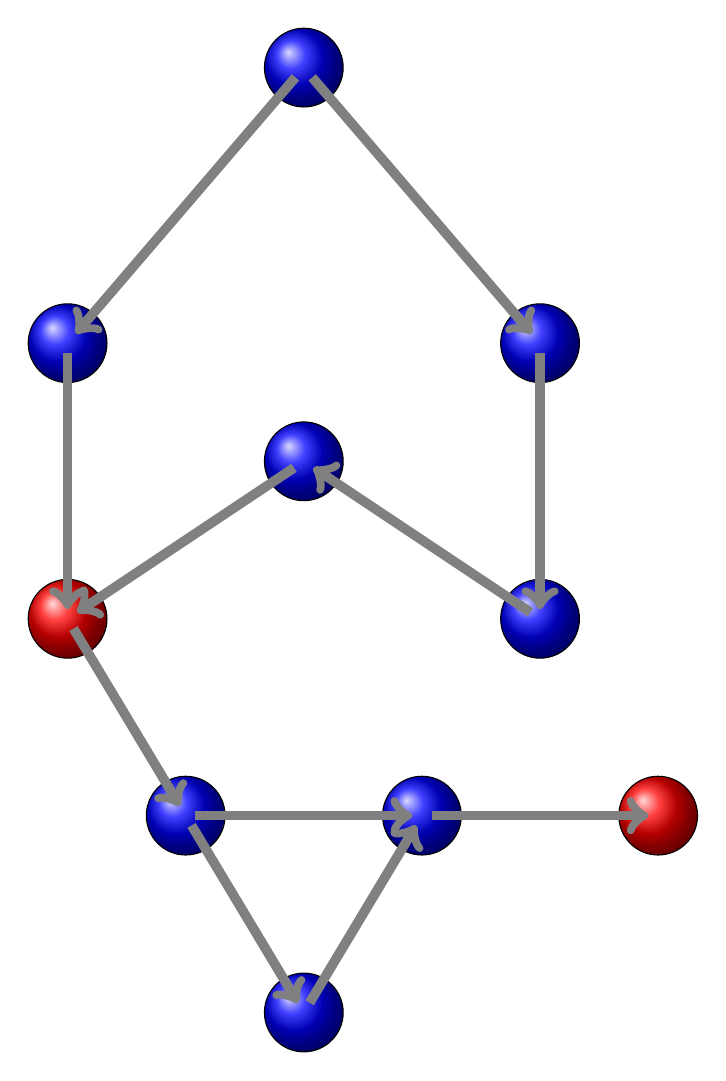
\begin{tikzpicture}
\draw[ball color=blue] (1,2) node (v3) {} circle (.5);
\draw[ball color=blue] (-2,-6.5) node (v9) {} circle (.5);
\draw[ball color=blue] (-0.5,-4) node (v8) {} circle (.5);
\draw[ball color=blue] (-3.5,-4) node (v7) {} circle (.5);
\draw[ball color=blue] (-2,0.5) node (v6) {} circle (.5);
\draw[ball color=blue] (1,-1.5) node (v5) {} circle (.5);
\draw[ball color=red] (-5,-1.5) node (v4) {} circle (.5);
\draw[ball color=blue] (-5,2) node (v2) {} circle (.5);
\draw[ball color=blue] (-2,5.5) node (v1) {} circle (.5);
\draw[ball color=red] (2.5,-4) node (v10) {} circle (.5);
\draw [->, draw=gray, line width=3.5] (v1) edge (v2)  (v1) edge (v3) (v2) edge (v4);
\draw [->, draw=gray, line width=3.5] (v3) edge (v5)  (v5) edge (v6) (v6) edge (v4) (v4) edge (v7);
\draw [->, draw=gray, line width=3.5] (v7) edge (v8)  (v7) edge (v9) (v9) edge (v8) (v8) edge (v10);
\end{tikzpicture}

\end{document}
